\documentclass[dvipsnames,crop=true]{standalone}
\usepackage{tikz}
\usetikzlibrary{calc,external,3d}
\begin{document}

  \tikzsetnextfilename{barrel_endcap}

  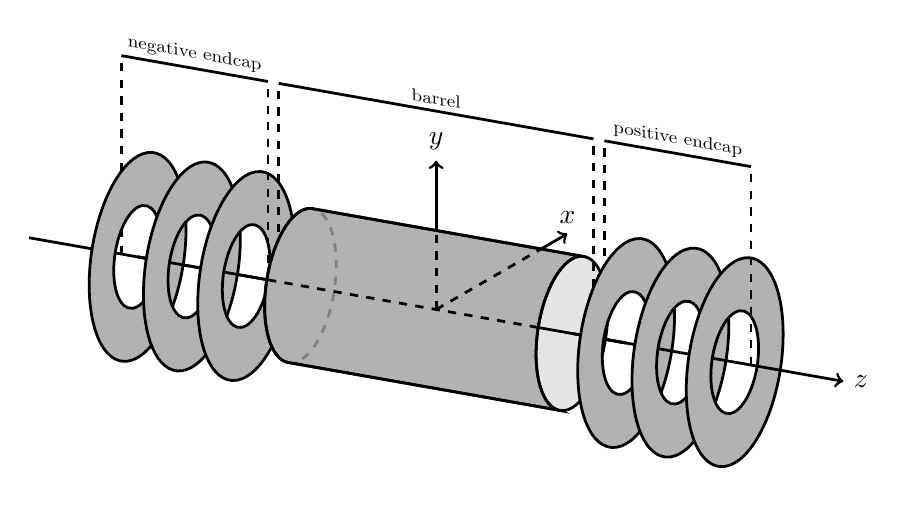
\begin{tikzpicture}[scale=0.7,line width=1pt]


  \begin{scope}[scale=1,x={(30:0.5cm)},y={(90:0.9cm)},z={(-10:1cm)}]
    \draw[->] (0,0,0) -- (5.5,0,0) node[at end,above] {$x$};
    \draw[->] (0,0,0) -- (0,3,0) node[at end,above] {$y$};
    \draw[-] (0,0,-7.5) -- (0,0,3.5);

    \coordinate(c0) at (0,0,-5);


    \def\n{10}
    \def\r{2}
    \pgfmathsetmacro{\ro}{\r+0.03}
    \pgfmathsetmacro{\ri}{\r-1}
    \def\dr{0.8}
    \pgfmathsetmacro{\da}{360/\n * 1}

    \def\o{4}
    \draw[dashed] (0,0,-5.8) --++(0,\o,0);

    \foreach \z [count=\j] in {%
      -5.5,%
      -4.5,%
      -3.5%
    } { 
      \coordinate (c\j) at (0,0,\z);

      \pgfmathsetmacro{\k}{int(\j-1)}
      \draw[] (c\k) -- (c\j);


      \begin{scope}[canvas is xy plane at z={\z}]
        \fill[black!30!white, even odd rule] (0,0) circle({\ro}) (0,0) circle({\ri});
        \draw[black] (0,0) circle({\ri}) (0,0) circle({\ro});
      \end{scope}
    }

    \draw[dashed] (0,0,-3.1) --++(0,\o,0);
    \draw[dashed] (0,0,-2.9) --++(0,\o,0);

    \draw (0,0,-3.5) -- (0,0,0);

    \def\rb{1.5}
    \def\aa{67}
    \def\ab{-113}
    \def\zb{-2.5}
    \def\zf{2.5}

    \begin{scope}[canvas is xy plane at z={\zb}]
      % \draw (\aa:\rb) arc(\aa:{\ab+360}:\rb);
      \coordinate (cba) at (\aa:\rb);
      \coordinate (cbb) at (\ab:\rb);
    \end{scope}

    \begin{scope}[canvas is xy plane at z={\zf}]
      % \draw (\aa:\rb) arc(\aa:{\ab+360}:\rb);
      \fill[black!10] (0,0) circle(\rb);
      \draw (\ab:\rb) arc(\ab:\aa:\rb);
      \coordinate (cfa) at (\aa:\rb);
      \coordinate (cfb) at (\ab:\rb);
    \end{scope}

    \draw (0,0,0) -- (0,0,3.5);

    \fill[black!30,draw=black] 
         ({cos(\aa)*\rb},{sin(\aa)*\rb},\zb)
      -- ({cos(\aa)*\rb},{sin(\aa)*\rb},\zf)
         arc(\aa:{\ab+360}:\rb)
      -- ({cos(\ab)*\rb},{sin(\ab)*\rb},\zb)
         arc({\ab+360}:{\aa}:\rb)
    ;

    \begin{scope}[canvas is xy plane at z={\zb}]
      \draw[dashed,black!50] (\ab:\rb) arc(\ab:\aa:\rb);
    \end{scope}

    \draw[] 
         ({cos(\aa)*\rb},{sin(\aa)*\rb},\zb)
      -- ({cos(\aa)*\rb},{sin(\aa)*\rb},\zf)
         arc(\aa:{\ab+360}:\rb)
      -- ({cos(\ab)*\rb},{sin(\ab)*\rb},\zb)
         arc({\ab+360}:{\aa}:\rb)
    ;

    \begin{scope}
      \clip
          ({cos(\aa)*\rb},{sin(\aa)*\rb},\zb)
        -- ({cos(\aa)*\rb},{sin(\aa)*\rb},\zf)
          arc(\aa:{\ab+360}:\rb)
        -- ({cos(\ab)*\rb},{sin(\ab)*\rb},\zb)
          arc({\ab+360}:{\aa}:\rb)
      ;

      % \fill[Red] (-10,-10) rectangle (10,10);
      \draw[dashed] (0,0,-4) -- (0,0,4);
      \draw[dashed,->] (0,0,0) -- (5,0,0);
      \draw[dashed,->] (0,0,0) -- (0,3,0);
      
    \end{scope}


    \draw[dashed] (0,0,2.9) --++(0,\o,0);
    \draw[dashed] (0,0,3.1) --++(0,\o,0);

    \coordinate(c0) at (0,0,\zf);

    \foreach \z [count=\j] in {%
      3.5,%
      4.5,%
      5.5%
      } {

      \pgfmathsetmacro{\jx}{int(\j+3)}

      \coordinate (c\j) at (0,0,\z);

      \pgfmathsetmacro{\k}{int(\j-1)}
      \draw[] (c\k) -- (c\j);


      \begin{scope}[canvas is xy plane at z={\z}]
        \fill[black!30!white, even odd rule] (0,0) circle({\ro}) (0,0) circle({\ri});
        \draw[black] (0,0) circle({\ri}) (0,0) circle({\ro});
      \end{scope}
    }

    \draw[->] (0,0,5.5) --++(0,0,2) node[at end,right] {$z$};

    \begin{scope}[canvas is zy plane at x=0]
      \draw [] (-2.9,\o) --++ ({2*2.9},0) node[midway,above,transform shape] {barrel};
      \draw [] (3.1,\o) -- (5.8,\o) node[midway,above,transform shape] {positive endcap};
      \draw [] (-3.1,\o) -- (-5.8,\o) node[midway,above,transform shape] {negative endcap};
    \end{scope}

    \draw[dashed] (0,0,5.8) --++(0,\o,0);


  \end{scope}


  \end{tikzpicture}

\end{document}